\documentclass[b4paper,10.5pt]{article}

\usepackage[UTF8]{ctex}
\usepackage{amsmath}
\usepackage{amssymb}
\usepackage{picins}

%-------------------------------------------------
% Article Start Now.
%-------------------------------------------------

\begin{document}

对于一个以圆心到极点的距离$a$为圆的半径的圆:\\

\begin{tabular}{lcl}
  % after \\: \hline or \cline{col1-col2} \cline{col3-col4} ...
  当圆心位于直线$\theta=0上时$ & 曲线方程为  & $\rho = 2a\cos \theta $ \\
  当圆心位于直线$\theta=\frac{\pi}{2}$上时 & 曲线方程为 & $\rho=2a\sin\theta $ \\
  当圆心位于直线$\theta=\pi$上时 & 曲线方程为 & $\rho=-2a\cos\theta $ \\
  当圆心位于直线$\theta=\frac{3\pi}{2}$上时 & 曲线方程为 & $\rho=-2a\sin\theta $ \\
\end{tabular}
\bigskip\bigskip

当圆心处于极坐标中任一位置时(如图所示),圆的一般形式方程为:\\
    \parpic[r]{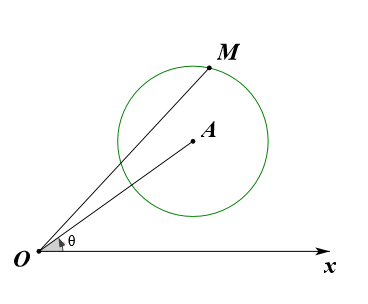
\includegraphics[width=0.35\textwidth]{C.png}}

设$A(\rho _{0},\theta _{0})$为圆心,$M(\rho,\theta)$为圆上任意一点,$r$为圆的半径:\\
则有$M(\rho,\theta)$的直角坐标表示为$M(\rho\cos\theta, \rho\sin\theta)$\\
$A(\rho_{0},\theta_{0})$的直角坐标表示为$A(\rho_0\cos\theta_0, \rho_0\sin\theta_0)$
$\therefore |AM|=\sqrt{(\rho\cos\theta-\rho_0\cos\theta_0)^2+(\rho\sin\theta-\rho_0\sin\theta_0)^2}$
即 $r^2=(\rho\cos\theta-\rho_0\cos\theta_0)^2+(\rho\sin\theta-\rho_0\sin\theta_0)^2$
$\therefore r^2=\rho^2\cos^2\theta+\rho_0^2\cos^2\theta_0-2\rho\rho_0\cos\theta\cos\theta_0 \\ +\rho^2\sin^2\theta+\rho_0^2\sin^2\theta_0-2\rho\rho_0\sin\theta\sin\theta_0$
$\therefore$
\begin{equation}\label{General Equ}
    r^2=\rho^2+\rho_0^2-2\rho\rho_0\cos(\theta-\theta_0)
\end{equation}
则曲线方程\ref{General Equ}即为圆在极坐标系中的一般方程.

总结:将极坐标化为直角坐标,使用圆上点到圆心距离始终相等来解决问题.

\end{document} 